%% This is an example first chapter.  You should put chapter/appendix that you
%% write into a separate file, and add a line \include{yourfilename} to
%% main.tex, where `yourfilename.tex' is the name of the chapter/appendix file.
%% You can process specific files by typing their names in at the 
%% \files=
%% prompt when you run the file main.tex through LaTeX.
\chapter{Conclusion}\label{chap:conclusion}
\section{Conclusion}
\subsection{Accomplishment}
In this thesis, I attempted to tackle the issue of detection, segmentation and tracking human hand from egocentric vision. Alongside investigating, affirming the hypothesis, and proposing a hand following by discovery framework, I built a module to detect and track human hands in videos from the first perspective. Chapter \ref{chap:intro} summarized the general overview of object recognition, including object classification, detection, segmentation and tracking in the wild and in the FPV. Related works are studied and discussed, associated project is also reported, and from that, the main problem is defined. Chapter \ref{chap:method} covers the background theory and methodology of the RCNN family and YOLO family, the SORT and DeepSORT algorithms.This chapter present and analyze egocentric hand datasets incorporate GTEA family, EgoHand; and furthermore present a new egocentric hand tracking datasets Micand32 alongside with a semi-automatic annotator EHTA. Chapter \ref{chap:framework} reported the proposed pipeline which contains 4 stage: data preparing stage, training stage, inference stage and evaluation stage. This chapter reports in detail techniques in the training and testing phase. Chapter \ref{chap:exp} describes about the evaluation criteria and then enumerates overall and featured detection, segmentation result following the COCO dataset standard and tracking result of 11 approaches on Micand32S and Micand32E following the MOT Challenge standard. Chapter \ref{chap:conclusion} terminates the thesis by considering the accomplishment, the drawback and also purpose some potential future works.
\subsection{Drawback}
Due to time constraints and limited human resource, the team hasn't completed labelling the whole datasets from Nafosted's project. The Micand32 dataset is completely new in terms of egocentric hand tracking and relatively good compared to other datasets in terms of sample size and labeling quality. However, due to many factors, this set is not general enough to train neural networks to function properly.

The number of experiments are relatively large, so I haven’t depthly analyzed the results. Algorithms work stably under laboratory conditions. In the wild, algorithms still have some problems to be solved, typically cases such as excessive arm resistance, long-term disappearance of an instance, blur effects at hand, the patient moves with a sudden acceleration, the abnormal movements of the patient’s hands.

Semi-automatic labeling tool needs users to know the basic code and observe to draw experience for each video to be assigned. The tool also works offline and has not integrated the online and real-time model update feature.

In terms of academics, the algorithms used in the thesis have not had new or breakthrough idea due to my shortcomings of expertise.
\section{Future works} \label{sec:futurework}
In this proposition, the meaning of the "hand" is ambiguous between datasets utilized. For GTEA family datasets, the "hand" incorporates the arm, wrist and hand while the "hand" in EgoHands datasets just contains only hand area and the "hand" in Micand32 isn't characterized obviously. This influences the nature of the egocentric hand re-identification dataset. Consequently, the deep appearance descriptor can't recognize the hand's highlights and doesn't function admirably. This re-identification dataset will be checked and upgraded in later works.

The EHTA framework currently works offline. An online annotation tool can update machine learning models right after the label adjustment of annotator. This will help the model predict better in the next frame as shown in Figure \ref{fig:future}. The EHTA pipeline is being developed to be more adaptable, flexible and productive. 
\begin{figure}[htbp]
	\centerline{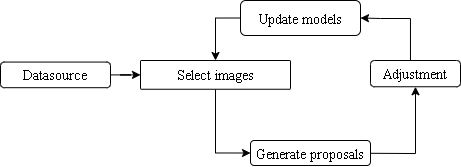
\includegraphics[width=0.5\textheight]{Figs/future.png}}
	\caption{Schematic illustration of an online annotation pipeline.}
	\label{fig:future}
\end{figure}

The remainder of the datasets in NAFOSTED’s project will be fully annotated. Algorithms then will be tested on this dataset. Likewise, other detection algorithms like SSD \cite{DBLP:journals/corr/LiuAESR15}, Retina \cite{8237586}, CenterNet \cite{9010985} and EfficientDet \cite{tan1911efficientdet} are being integrated and tested.

As a relative complicated and integrated computer vision mission like multiple object tracking, the tracking by detection technique referenced in this thesis is still suffering from issues such as a large number of false positive tracks. False positive tracks caused by unreliable detection results are badly affecting the performance of trackers. To reduce the effect of unreliable detection on tracking, in the future works, I propose to incorporate a low confidence track filtering extension into DeepSORT. Tracks with low average detection confidence in their initial several frames will be deleted. This strategy is promising and it has been conducted on a vehicle tracking problem \cite{8909903} similar to this thesis.

The accelerometer sensors worn by patients generate real-time kinetics information \cite{4651201}. This acceleration information is extremely useful and can be fed to Kalman filter to predict the motion model better. I propose to match the sensor stream from the accelerometer with the camera to detect instances of the hand’s physical movement. This method has a wide range of potential applications in the cyber-physical systems domain such as identification, localization, tracking and action recognition, for example, Leap Motion \cite{8711887} is a well-known and successful commercial product designed for hand tracking in virtual reality.